不必要的对象复制可能是C++的低效之处。主要原因是这样做很简单,但很难关注到。看一下以下代码:

\begin{lstlisting}[style=styleCXX]
std::vector<int> v = make_v(… some args …);
do_work(v);
\end{lstlisting}

这个程序中,\texttt{v}被复制了多少次?答案取决于\texttt{make\_v()}和\texttt{do\_work()}函数的实现以及编译器的优化。这个例子涵盖了我们现在要讨论的一些语言细节。

\subsubsubsection{9.3.1\hspace{0.2cm}复制和参数传递}

我们将从第二个函数\texttt{do\_work()}开始。若函数以引用(\texttt{const}或非\texttt{const}形式)传递实参,则不进行复制。

\begin{lstlisting}[style=styleCXX]
void do_work(std::vector<int>& vr) {
	… vr is a reference to v …
}
\end{lstlisting}

若函数使用按值传递,则必须进行复制:

\begin{lstlisting}[style=styleCXX]
void do_work(std::vector<int> vc) {
	… vc is a copy of v …
}
\end{lstlisting}

如果\texttt{vector}对象很大,则复制\texttt{vector}对象的操作代价很高:必须复制\texttt{vector}对象中的所有数据,这是一个代价很高的函数调用。如果不需要\texttt{vector}的副本,那么这里的复制就非常的低效。例如,如果只需要计算\texttt{vector}中所有元素的和(或其他计算),则不需要副本。乍一看,调用本身并没有告诉我们是否复制,但它应该是这样的。复制的决定属于函数的实现者,只有在考虑了需求和算法的选择后才能做出。对于前面提到的累加所有元素和的问题,正确的决定显然是通过(\texttt{const})引用传递\texttt{vector}对象,如下所示:

\begin{lstlisting}[style=styleCXX]
void do_work(const std::vector<int>& v) {
	int sum = 0;
	for (int x: v) sum += x;
	… use sum … 
}
\end{lstlisting}

这种情况下,使用值传递明显是低效的,并可能会认为是一个Bug,但是这种情况发生的频率比还挺高。特别是在模板代码中,作者只考虑了小型、轻量级的数据类型,但代码最终得到了比预期更广泛的使用。

另一方面,如果需要创建实参的副本,作为满足函数要求的一部分,使用参数传递是一种很好的方法:

\begin{lstlisting}[style=styleCXX]
	void do_work(std::vector<int> vc) {
		… vc is a copy of v …
	}
\end{lstlisting}

进一步处理数据之前,我们需要对数据应用一个所谓的固定环。假设多次读取固定位的值,每次访问都调用\texttt{std::min()}可能比创建结果的缓存副本的效率要低。我们也可以显式的制作一个副本,这可能会更有效,但这种优化不应该只是猜测,需要通过一个基准测试才能明确回答。

C++11引入了移动语义来解决部分不必要的复制。本例中,我们观察到,如果函数实参是右值,可以以任何方式使用它,包括修改它(调用者在调用完成后无法访问该对象)。利用移动语义的常用方法是使用右值引用版本重载函数:

\begin{lstlisting}[style=styleCXX]
void do_work(std::vector<int>&& v) {
	… can alter v data … 
}
\end{lstlisting}

但是,如果对象本身支持移动,简单的值传递版本就有了亮点。参考以下代码:

\begin{lstlisting}[style=styleCXX]
void do_work(std::vector<int> v) {
	… use v destructively … 
}
std::vector<int> v1(…);
do_work(v1);                 // Local copy is made
do_work(std::vector<int>(…));    // rvalue
\end{lstlisting}

\texttt{do\_work()}的第一次调用使用了左值参数,因此在函数内部进行了局部复制(参数通过值传递!)。第二个调用使用右值或未命名的临时函数,由于\texttt{vector}有一个移动构造函数,函数的实参移动(而不是复制!)到形参中,移动\texttt{vector的}速度非常快。现在,在没有任何重载的情况下,通过函数实现,可以有效地处理右值和左值参数,现在我们已经看到了两个极端的例子。第一种情况下,不需要副本,显式的构造一份是低效的。第二种情况下,复制是一种合理的实现。正如我们即将看到的,并不是每一种情况都属于这些极端情况。

\subsubsubsection{9.3.2\hspace{0.2cm}使用复制进行实现}

还有一种中间情况,即选择的实现需要参数的副本,但实现本身并不是最优的。例如,考虑下面的函数,它需要按顺序输出向量:

\hspace*{\fill} \\ %插入空行
\noindent
\textbf{01\_vector\_sort.C}
\begin{lstlisting}[style=styleCXX]
void print_sorted(std::vector<int> v) {
	std::sort(v.begin(), v.end());
	for (int x: v) std::cout << x << “\n”;
}
\end{lstlisting}

对于一个整数\texttt{vector},这可能是最好的方法,我们对容器本身进行排序并按顺序打印。因为不应该修改原始容器,所以需要一个副本,而且需要利用编译器来创建一个副本也没有什么错。

但是如果\texttt{vector}的元素不是整数,而是一些大型对象呢?在这种情况下,复制\texttt{vector}就需要占用大量内存,而对其进行排序需要花费大量时间来复制大型对象。这种情况下,更好的实现可能是在不移动原始对象的情况下,创建指针\texttt{vector}并对其排序:

\hspace*{\fill} \\ %插入空行
\noindent
\textbf{01\_vector\_sort.C}
\begin{lstlisting}[style=styleCXX]
template <typename T>
void print_sorted(const std::vector<T>& v) {
	std::vector<const T*> vp; vp.reserve(v.size());
	for (const T& x: v) vp.push_back(&x);
	std::sort(vp.begin(), vp.end(), 
		[](const T* a, const T* b) { return *a < *b;});
	for (const T* x: vp) std::cout << *x << “\n”;
}
\end{lstlisting}

因为我们现在已经学会了永远不要猜测性能,所以直觉需要通过基准测试来确认。因为对已经排序的\texttt{vector}进行排序不需要任何复制,所以我们希望在基准测试的每次迭代中都有一个新的、未排序的\texttt{vector},如下所示:

\hspace*{\fill} \\ %插入空行
\noindent
\textbf{01\_vector\_sort.C}
\begin{lstlisting}[style=styleCXX]
void BM_sort(benchmark::State& state) {
	const size_t N = state.range(0);
	std::vector<int> v0(N); for (int& x: v0) x = rand();
	std::vector<int> v(N);
	for (auto _ : state) {
		v = v0;
		print_sorted(v);
	}
	state.SetItemsProcessed(state.iterations()*N);
}
\end{lstlisting}

当然,我们应该禁用打印,因为我们对I/O基准测试不感兴趣。另一方面,我们应该在不进行排序的情况下对复制\texttt{vector}进行基准测试,这样就可以知道所测量的时间的哪一部分花在了准备测试上。

基准测试确认,对于整数,复制整个\texttt{vector}对象并对其进行排序会更快:

%\hspace*{\fill} \\ %插入空行
\begin{center}
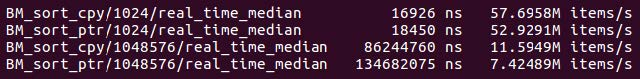
\includegraphics[width=0.9\textwidth]{content/3/chapter9/images/1.jpg}\\
图9.1 - 对一个整数\texttt{vector}排序的基准测试:复制方式和指针方式(间接)的对比
\end{center}

请注意,如果向量很小,而且所有数据都适合底层缓存,那么无论哪种方式,处理速度都非常快,而且速度差异很小。如果对象比较大,复制的代价也比较高,那么间接性方式就会比较高效:

%\hspace*{\fill} \\ %插入空行
\begin{center}
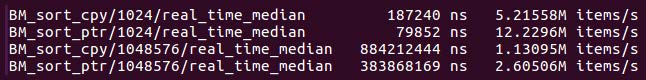
\includegraphics[width=0.9\textwidth]{content/3/chapter9/images/2.jpg}\\
图9.2 - 大型对象的\texttt{vector}排序基准测试:复制方式和指针(间接)方式
\end{center}

还有一种特殊情况,即实现时需要复制对象。这个,我们下次再讨论。

\subsubsubsection{9.3.3\hspace{0.2cm}复制存储数据}

In C++, we can encounter another particular case of data copying. It happens most often in class constructors where the object must store a copy of the data, so a long-term copy with a lifetime exceeding that of the constructor call must be created. Consider this example:

\begin{lstlisting}[style=styleCXX]
class C {
	std::vector<int> v_;
	C(std::vector<int> ??? v) { … v_ is a copy of v … }
};
\end{lstlisting}

Here the intent is to make a copy. The inefficiency would be to make multiple intermediate copies or make an unnecessary copy. The standard way to accomplish this is to take the object by const reference and make a copy inside the class:

\begin{lstlisting}[style=styleCXX]
class C {
	std::vector<int> v_;
	C(const std::vector<int>& v) : v_(v) { … }
};
\end{lstlisting}

If the argument of the constructor is an lvalue, this is as efficient as it can be. However, if the argument is an rvalue (a temporary), we would prefer to move it into the class and make no copies at all. This requires an overload for the constructor:

\begin{lstlisting}[style=styleCXX]
class C {
	std::vector<int> v_;
	C(std::vector<int>&& v) : v_(std::move(v)) { … }
};
\end{lstlisting}

The downside is the need to code two constructors, but it gets worse if the constructor takes several arguments, and each one needs to be copied or moved. Following this pattern, we would need 6 constructor overloads to handle 3 parameters.

The alternative is to pass all parameters by value and move from the parameter, check the following code:

\begin{lstlisting}[style=styleCXX]
class C {
	std::vector<int> v_;
	C(std::vector<int> v) : v_(std::move(v)) 
	{ … do not use v here!!! … }
};
\end{lstlisting}

It is very important to remember that the parameter v is now an object in a moved-from state, and it should not be used in the body of the constructor. If the argument is an lvalue, a copy is made to construct the parameter v, then moved into the class. If the argument is an rvalue, it is moved into the parameter v and again moved into the class. This pattern works great if the objects are cheap to move. However, if the objects are expensive to move or have no move constructors at all (so they are copied instead), we end up doing two copies instead of one. 

So far, we have focused on the problem of getting data into functions and objects. But copying can also occur when we need to return the results. The considerations there are completely different and need to be examined separately

\subsubsubsection{9.3.4\hspace{0.2cm}Copying of return values}

Our example at the very beginning of this section included both kinds of copying. In particular, this line:

\begin{lstlisting}[style=styleCXX]
std::vector<int> v = make_v(… some args …);
\end{lstlisting}

It implies that the resulting vector v is created from another vector, the one returned by the function make\_v:

\hspace*{\fill} \\ %插入空行
\noindent
\textbf{02\_rvo.C}
\begin{lstlisting}[style=styleCXX]
std::vector<int> make_v(… some args …) {
	std::vector<int> vtmp;
	… add data to vtmp …
	return vtmp;
}
\end{lstlisting}

In theory, more than one copy can be made here: the local variable vtmp is copied into the (unnamed) return value of the function make\_v, which is, in turn, copied into the final result v. In practice, this is not going to happen. First of all, the unnamed temporary return value of make\_v is moved, not copied, into v. But, most likely, even this is not going to happen. If you try this code with your own class instead of std::vector, you will see that neither a copy nor a move constructor is used:

\hspace*{\fill} \\ %插入空行
\noindent
\textbf{02\_rvo.C}
\begin{lstlisting}[style=styleCXX]
class C {
	int i_ = 0;
	public:
	explicit C(int i) : i_(i) { 
		std::cout << “C() @” << this << std::endl;
	}
	C(const C& c) : i_(c.i_) {
		std::cout << “C(const C&) @” << this << std::endl;
	}
	C(C&& c) : i_(c.i_) {
		std::cout << “C(C&&) @” << this << std::endl;
	}
	~C() { cout << “~C() @” << this << endl; }
	friend std::ostream& operator<<( std::ostream& out,
	const C& c) {
		out << c.i_; return out;
	}
};  
C makeC(int i) { C ctmp(i); return ctmp; }
int main() {
	C c = makeC(42);
	cout << c << endl;
}
\end{lstlisting}

This program prints something like the following (on most compilers, a certain level of optimization must be turned on):

\hspace*{\fill} \\ %插入空行
\begin{center}
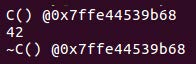
\includegraphics[width=0.9\textwidth]{content/3/chapter9/images/3.jpg}\\
Figure 9.3 – The output of the program returning an object by value
\end{center}

As you can see, only one object was constructed and destroyed. This is the result of the compiler optimization. The specific optimization that is used here is known as Return Value Optimization (RVO). The optimization itself is very simple: the compiler recognized that the three objects involved – the local variable ctmp, the unnamed temporary return value, and the final result c – are all of the same type. Furthermore, it is impossible for any code we write to observe any two of these variables at the same time. Therefore, without changing any observable behavior, the compiler can use the same memory location for all three variables. Before calling the function, the compiler needs to allocate the memory where the eventual result c will be constructed. The address of this memory is passed into the function by the compiler, where it is used to construct the local variable ctmp at the same location. As a result, when the function makeC ends, there is nothing to return at all: the result is already where it should be. This is the RVO in a nutshell.

While RVO seems simple, it has several subtleties. 

First, remember that this is an optimization. This means that the compiler usually does not have to do it (if yours doesn’t, you need a better compiler). However, it is a very special kind of optimization. In general, the compiler can do whatever it wants to your program as long as it does not change the observable behavior. The observable behavior includes input and output and accessing volatile memory. This optimization, however, has resulted in an observable change: the expected output of the copy constructor and the matching destructor is nowhere to be seen. Indeed, this is one exception from the otherwise ironclad rule: the compiler is allowed to eliminate calls to copy or move constructors and the corresponding destructors even if these functions have side effects that include observable behavior. This exception is not limited to RVO. The implication is that, in general, you cannot count on copy and move constructors to be called just because you wrote some code that appears to do a copy. This is known as copy elision (or move elision, for move constructors).

Second, remember (again) that this is an optimization. The code must compile before it can be optimized. If your object does not have any copy or move constructors, this code will not compile, and we will never get to the optimization step that is going to remove all calls to these constructors. This is easy to see if we delete all copy and move constructors in our example:

\begin{lstlisting}[style=styleCXX]
class C {
	…
	C(const C& c) = delete;
	C(C&& c) = delete;
}; 
\end{lstlisting}

The compilation will now fail. The exact error message depends on the compiler and the C++ standard level; in C++17, it is going to look something like this:

\hspace*{\fill} \\ %插入空行
\begin{center}
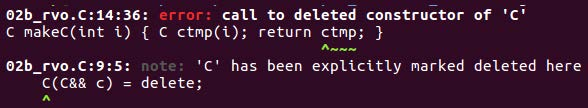
\includegraphics[width=0.9\textwidth]{content/3/chapter9/images/4.jpg}\\
Figure 9.4 – Compilation output of Clang using C++17 or C++20
\end{center}

There is one special case where our program would compile even with deleted copy and move operations. Let us make a slight change to the makeC function:

\begin{lstlisting}[style=styleCXX]
C makeC(int i) { return C(i); }
\end{lstlisting}

Nothing changes in C++11 or C++14; however, in C++17 and above, this code compiles fine. Note the slight difference from the previous version: the returned object used to be an lvalue, it had a name. Now it’s an rvalue, an unnamed temporary. This makes all the difference: while the named RVO (NRVO) is still an optimization, the unnamed RVO is mandatory since C++17 and is no longer considered to be a copy elision. Instead, the standard says that no copy or move is requested in the first place. 

Finally, you may wonder if the function must be inlined in order for the compiler to know where the return value is while it compiles the function itself. With a simple test, you can convince yourself that this is not so: even if the function makeC is in a separate compilation unit, RVO still takes place. The compiler, therefore, must send the address of the result to the function at the call point. You can do something similar yourself if you do not return the result from the function at all but instead pass the reference to the result as an additional argument. Of course, that object has to be constructed first, while the compiler-generated optimization does not need an extra constructor call. 

You may find a recommendation to not rely on RVO but to enforce the move of the return value instead:

\begin{lstlisting}[style=styleCXX]
C makeC(int i) { C c(i); return std::move(c); }
\end{lstlisting}

The argument goes that if RVO does not happen, your program will take the performance penalty of the copying operation, while the move operation is cheap anyway. However, this argument is wrong. To understand why, look carefully at the error message in Figure 9.4: the compiler complains that the move constructor is deleted even though ctmp is an lvalue and should be copied. This is not a compiler bug but reflects the behavior required by the standard: in the context where the return-value optimization is possible, but the compiler decides not to do it, the compiler must first try to find a move constructor to return the result. If the move constructor is not found, the second lookup is performed; this time, the compiler is looking for a copy constructor. In both cases, the compiler is really performing overload resolution since there can be many copy or move constructors. Thus, there is no reason to write an explicit move: the compiler will do one for us. But what is the harm, then? The harm is that using the explicit move disables RVO; you have asked for a move, so you are going to get one. While a move may require very little work, RVO is no work at all, and no work is always faster than some work.

What happens if we delete the move constructor but not the copy constructor? The compilation still fails in the case where it was failing with both constructors deleted. This is, again, a subtle point of the language: declaring a deleted member function is not the same as not declaring any. If the compiler performs the overload resolution for a move constructor, it will find one, even if this constructor is deleted. The compilation fails because the overload resolution selected a deleted function as the best (or the only) overload. If you want to force the use of the copy constructor (in the name of science, of course), you have to not declare any move constructors at all. 

By now, you must see the danger of accidentally copying an object and ruining your program’s performance hiding behind every dark corner of your code. What can you do to avoid unintentional copying? We will have some suggestions in a moment, but first, let us return to one approach that we already used briefly: the use of pointers.

\subsubsubsection{9.3.5\hspace{0.2cm}Using pointers to avoid copying}

One way to avoid copying objects when passing them around is to pass pointers instead. This is easiest if we don’t have to manage the object’s lifetime. If a function needs access to an object but does not need to delete it, passing the object by reference or by a raw pointer is the best way (the reference, in this context, is really just a pointer that cannot be null). 

Similarly, we can return an object from a function using a pointer, but this needs more care. First of all, the object must be allocated on the heap. You must never return pointers or references to local variables. Refer to the following code:

\begin{lstlisting}[style=styleCXX]
C& makeC(int i) { C c(i); return c; } // Never do this!
\end{lstlisting}

Second, the caller is now responsible for deleting the object, so every caller of your function must know how the object was constructed (operator new is not the only way to construct objects, just the most common one). The best solution here is to return a smart pointer:

\hspace*{\fill} \\ %插入空行
\noindent
\textbf{03\_factory.C}
\begin{lstlisting}[style=styleCXX]
std::unique_ptr<C> makeC(int i) {
	return std::make_unique<C>(i);
}
\end{lstlisting}

Note that such a factory function should return unique pointers even if the caller may use shared pointers to manage the object’s lifetime: it is easy and cheap to move from the unique pointer to the shared one.

Speaking of shared pointers, they are often used to pass around objects whose lifetime is managed by smart pointers. Unless the intent is to pass the ownership of the object as well, this is again an example of unnecessary and inefficient copying. Copying shared pointers is not cheap. So, what do we do if we have an object managed by a shared pointer and a function that needs to operate on this object without taking ownership of it? We use raw pointers:

\begin{lstlisting}[style=styleCXX]
void do_work1(C* c);
void do_work2(const C* c);
std::shared_ptr<C> p { new C(…) };
do_work1(&*p);
do_work2(&*p);
\end{lstlisting}

The declarations of the functions do\_work1() and do\_work2() tell us about the programmer’s intent: both functions operate the object without deleting it. The first function modifies the object; the second does not. Both functions expect to be called without the object and will handle this special case (otherwise, the arguments would be passed by reference). 

Similarly, you can create containers of raw pointers as long as the lifetime of the objects is managed elsewhere. If you want the container to manage the lifetime of its elements but do not want to store the objects in the container, a container of unique pointers will do the job. 

Now it is time for some general guidelines that will help you avoid unnecessary copying and the inefficiencies it can cause.

\subsubsubsection{9.3.6\hspace{0.2cm}How to avoid unnecessary copying}

Perhaps the most important thing you can do to reduce accidental, unintentional copying is to ensure that all your data types are movable if moving can be implemented cheaper than copying. If you have container libraries or other reusable code, make sure it is move-enabled as well. 

The next suggestion is somewhat hamfisted, but it can save you a lot of debugging time: if you have types that are expensive to copy, make them non-copyable to begin with. Declare the copy and assignment operations as deleted. If the classes support a fast move, provide move operations instead. This will, of course, prevent any copying, intentional or not. Hopefully, intentional copying is rare, and you can implement a special member function like clone() that will create a copy of the object. At least this way, all the copying is explicit and visible in your code. If the class is neither copyable nor movable, you will not be able to use it with STL containers; however, a container of unique pointers is a fine alternative. 

When passing parameters to functions, use references or pointers whenever possible. If the function needs to make a copy of the argument, consider passing by value and moving from the parameter instead. Remember that this works well only for move-enabled types, and see the first guideline.

Everything we said about passing function arguments can be applied to temporary local variables as well (after all, function parameters are basically temporary local variables in the function scope). These should be references unless you need a copy. This does not apply to the built-in types like integers or pointers: they are cheaper to copy than to access indirectly. In template code, you don’t have the luxury of knowing whether the type is large or small, so use references and rely on compiler optimizations to avoid unnecessary indirect access to built-in types.

When returning values from functions, your first preference should be to rely on RVO and copy elision. Only when you find that the compiler does not perform this optimization and that it matters in your particular case should you consider alternatives. These alternatives are: using functions with output arguments and using factory functions that construct the results in dynamically allocated memory and return owning smart pointers such as std::unique\_ptr. 

Finally, review your algorithms and the implementation with an eye out for unnecessary copying: remember that ill-intentioned copying is just as bad for the performance as unintentional copying.

We are done with the first bane of efficiency in C++ programs, the gratuitous copying of objects. The close second is poor memory management.














